\documentclass{tufte-handout}
\usepackage{braph2_tut}
%\geometry{showframe} % display margins for debugging page layout

\title{Brain Atlas}

\author[The BRAPH~2 Developers]{The BRAPH~2 Developers}

\begin{document}

\maketitle

\fig{figure*}
	{fig:xxx}
	{
	[b!]
	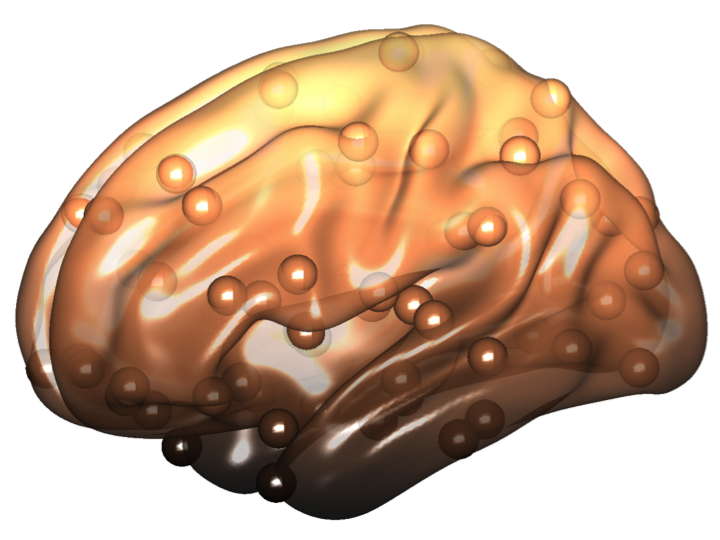
\includegraphics{tut_ba/fig1.png}
	}
	{Brain Atlas GUI.}
	{
	Graphical user interface to work with brain atlases. 
	}
	
\begin{abstract}
\noindent
This is the tutorial for working with the Graphical User Interface of Brain Atlas, the first step to perform an analysis in BRAPH 2.0. 
In this Tutorial, we will explain how to create a new atlas or upload an atlas that is already prepared for you to run an analysis.
\end{abstract}

%%%%% %%%%% %%%%% %%%%% %%%%%
\clearpage
\section{Example figures}

\fig{marginfigure}
	{fig:xxx}
	{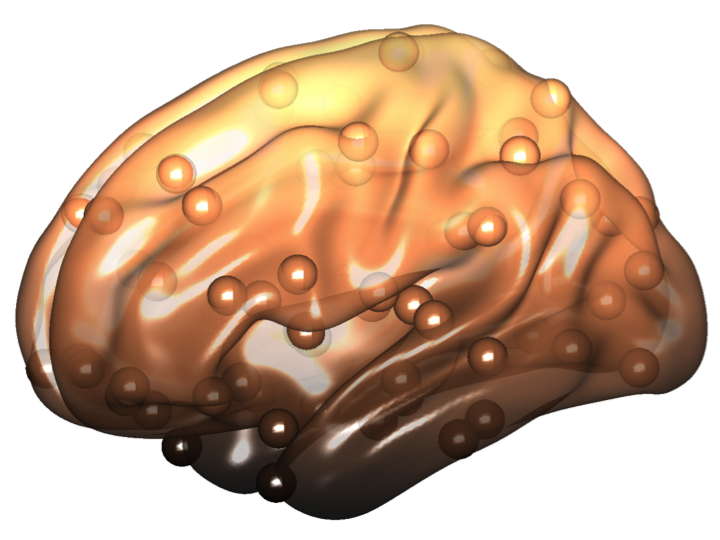
\includegraphics{tut_ba/fig1.png}}
	{TITLE}
	{
	caption
	}

\fig{figure}
	{fig:xxx}
	{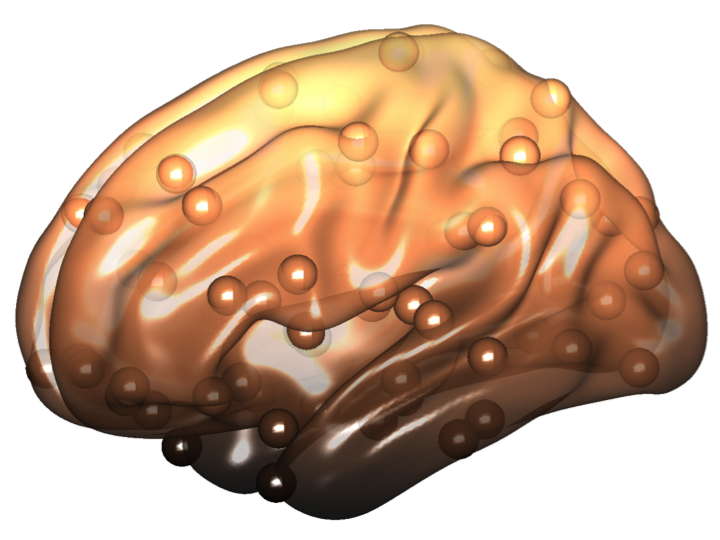
\includegraphics{tut_ba/fig1.png}}
	{TITLE}
	{
	caption
	}

\fig{figure*}
	{fig:xxx}
	{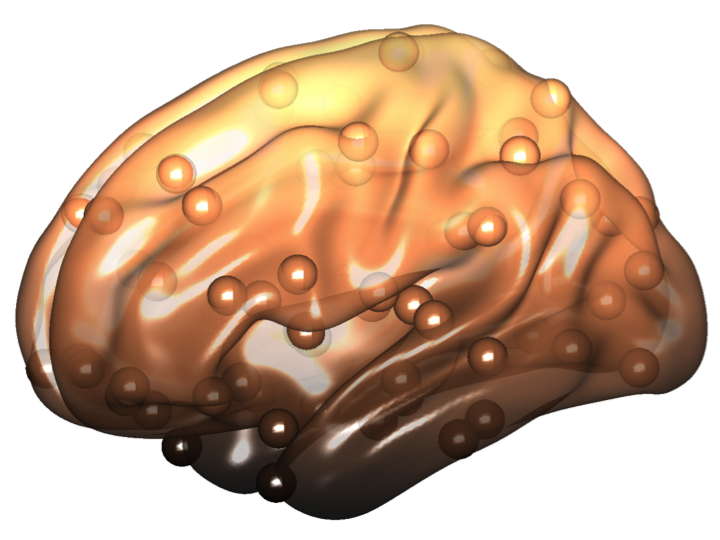
\includegraphics{tut_ba/fig1.png}}
	{TITLE}
	{
	caption
	}


%%%%% %%%%% %%%%% %%%%% %%%%%
\clearpage
\section{Prepared Brain Atlases}

Currently we provide the following brain atlas, which can be downloaded at: http://braph.org/software/brain-atlases/:


- AAL90 (automated anatomical labeling with 90 regions)


- AAL116 (automated anatomical labeling with 116 regions)


- BNA (Brainnetome with 246 regions)


- Craddock (functional atlas with 200 regions)


- Desikan (anatomical atlas with 68 cortical and 14 subcortical gray matter regions from the FreeSurfer software)


-  Destrieux (anatomical atlas with 148 cortical and 14 subcortical gray matter regions from the FreeSurfer software)


- Schaefer (functional brain atlas with 200 regions that belong to 7 different resting-state networks)


\section{Create a New Brain Atlas}

To prepare a Brain Atlas in BRAPH 2.0 format, you should open a new excel file (.xls or .xlsx) and write the following information in the first 4 rows:

- Brain Atlas ID (row 1, column 1)
For example: Desikan FreeSurfer


- Brain Atlas LABEL (row 2, column 1)
For example: Desikan FreeSurfer Labels


- Brain Atlas NOTES (row 3, column 1)
For example: Desikan FreeSurfer Nodes


- Brain Surface Name (row 4, column 1)
For example: BrainMeshICBM152.nv


Then, from row 5, you should include the short IDs of the regions of your atlas (1st column), the full Labels of the  regions of your atlas (2nd column), the x, y and z coordinates (3rd, 4th and 5th columns), the brain hemisphere (6th column). Take a look at the following snapshot for a quick overview of this information:







the generator file \fn{*.gen.m} for a new measure which can the be compiled by \code{braph2genesis}, using the measures \code{Degree}, \code{DegreeAv}, and \code{Distance} as examples.

\tableofcontents

%%%%% %%%%% %%%%% %%%%% %%%%%
\clearpage
\section{Implementation of Degree}

xxx

\subsection{Implementation of Degree}

\begin{enumerate}
\item
\item
\end{enumerate}

%\bibliography{biblio}
%\bibliographystyle{plainnat}

\end{document}